\chapter{Konzeption}
\label{cha:konzeption}
Bei der Konzeption wurde der aktuelle Stand des bestehenden Webauftritts betrachtet und analysiert. Im weiteren Schritt wurden Erweiterungen für die Website geplant. Im nächsten großen Schritt erfolgte eine Analyse aktuell bestehender Software, welche Gegenstände verwaltet.


\section{Analyse des aktuellen Webauftritts}
\label{webauftritt}
Der Webauftritt, erreichbar im Netzwerk der Hochschule Furtwangen\url{http://web.smarthome.hs-furtwangen.de/}, des \ac{SHL} Labors, wird mit der Hilfe des \ac{CMS} WordPress verwaltet. WordPress eigne sich hier, weil es mittels \ac{UX} so gestaltet wurde, das es sehr leicht zu erlernen ist. Unerfahrene Benutzer könne so schnell eigene Inhalte einpflegen.

\begin{figure}[bh]
	\centering
	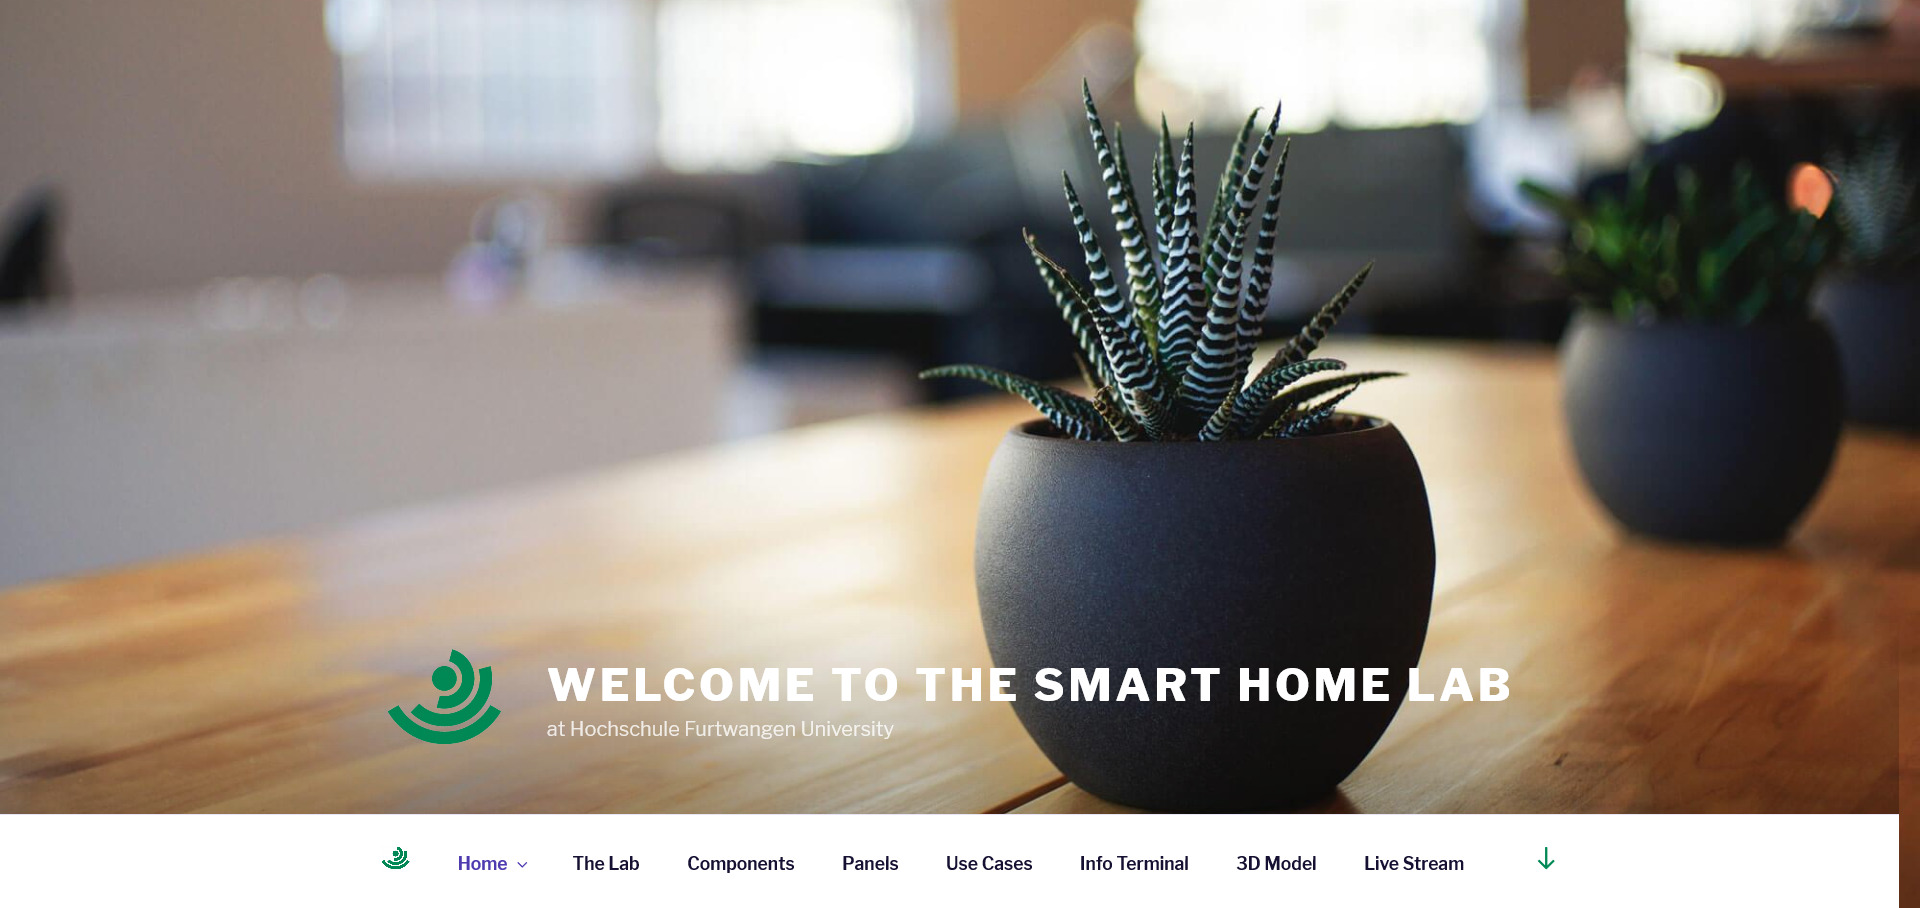
\includegraphics[scale=0.23]{content/pictures/shlwebsit.jpg}
	% bosch_iot_poll.png: 0x0 pixel, 300dpi, 0.00x0.00 cm, bb=
	\caption{Die Startseite des Webauftritts}
	\label{fig:web}
\end{figure}

Die Website ist mit dem, von WordPress eigenem Designe Twentyseventeen gestaltet. Auf der Startseite sieh man ein großes Headerbild. Darunter Folgt eine Navigationsleiste, welche die Links bei einem Besuch einer Unterseite in einem Lila Farbton darstellt. Die Navigation umfasst die Seiten:

\begin{itemize}
	\item Home
	
	\item The Lab 
	
	\item Components 
	
	\item Panels
	
	\item Use Cases 
	
	\item Info Terminal
	
	\item 3D Model
	
	\item Live Stream
	
	
	
\end{itemize}

Weiter folgt eine kurze Beschreibung über das Labor. Der nächste Abschnitt der Startseite stellt das Team vor. Im Anschluss sieht man noch ein Video, welches das Labor vorstellt, ein Kontaktforumlar und die Addresse mit einer Google Maps Karte. Am untersten Ende ist ein Footer, welche eine Copyright und einen Link zum Impressum enthält.

Die Unterseite "The Lab" stellt das Labor mit Grundrissen etwas detailreicher vor. "Components" stellt wenige, aber wichtige Geräte vor. In "Panels" werden, die mit Sensoren und Geräte versehenen, Wände in den Räumen beschrieben. Eine Auswahl von umgesetzten Anwendungsfällen werden in der Unterseite "Use Cases" beschrieben. Für das Infoterminal gibt es ebenfalls eine Unterseite, welche automatisiert eine Präsentation über das Labor abspielt. Unter dem Punkt "3D Model", befindet sich eine 3D Ansicht des Labors, welches sich in einer Ego- und Vogelperspektive betrachten lässt. Auch können hier vereinzelt Geräte bedient werden. Abgeschlossen wird die Navigation mit einer Unterseite, welche einen Video Livestream zeigen kann.

 

\subsection{Corporate Design}
Mit den aktuellen Farben entspricht der Webauftritt des Labors nicht dem \ac{CD} der Hochschule Furtwangen. So müssen die Lila Farben durch die Farbe Grün mit dem Hexwert 83b62d geändert werden. Dies ist wichtig um einen Wiedererkennungswert der Hochschule darzustellen. Die Navigation stellte hier einen größeren Bruch dar. Um die Seite vollständig im \ac{CD} der Hochschule zu haben, ist ein Expertengespräch nötig.



\subsection{Erweiterung des Webauftritts}
Neben dem \acf{CD} gab es noch weitere Punkte, welche den Auftritt noch Informativer und attraktiver gestalten konnten. So stehen im Labor die einzelnen Räume: Küche, Bad, Multimediaraum, IoT-Raum und der Arbeitsbereich stark im Vordergrund. Diese wurden bisher nur sehr dürftig auf der Homepage erwähnt.

\section{Konzeption des Inventarisierungssystem}
\label{inventar}


\section{Vergleichbare Inventarisierungssysteme}

\subsection{Anforderungen}


\subsection{Scrum}

\subsection{Datenbank}

\subsection{MockUps}

\subsection{User Experience}

\subsection{Fitts Gesetze}

\section{Wahl der Frameworks}
